% The real pairing schedule of the September Sonnet 4.5 population run rep00
% (negative_only_reasoning_rerun_population_myth_game_claude_n5 /
% noisy8_crossmodel_negative_twotask_r3; the same schedule is used by the GPT-5 Nano
% and Gemini 3.7 Flash reps of the same index, because pairing seeds are paired).
% Solid orange: the four trust games of a round (arrow from sender to receiver).
% Dashed: where each myth goes - to the writer's game partner of that round, who
% reads it in the next round. Filled nodes: agents whose current myth descends
% from Agent 1's founding (round-1) myth.
\documentclass[tikz,border=8pt]{standalone}
\usepackage[T1]{fontenc}
\usepackage{lmodern}
\renewcommand{\familydefault}{\sfdefault}
\usetikzlibrary{arrows.meta,calc}
\begin{document}
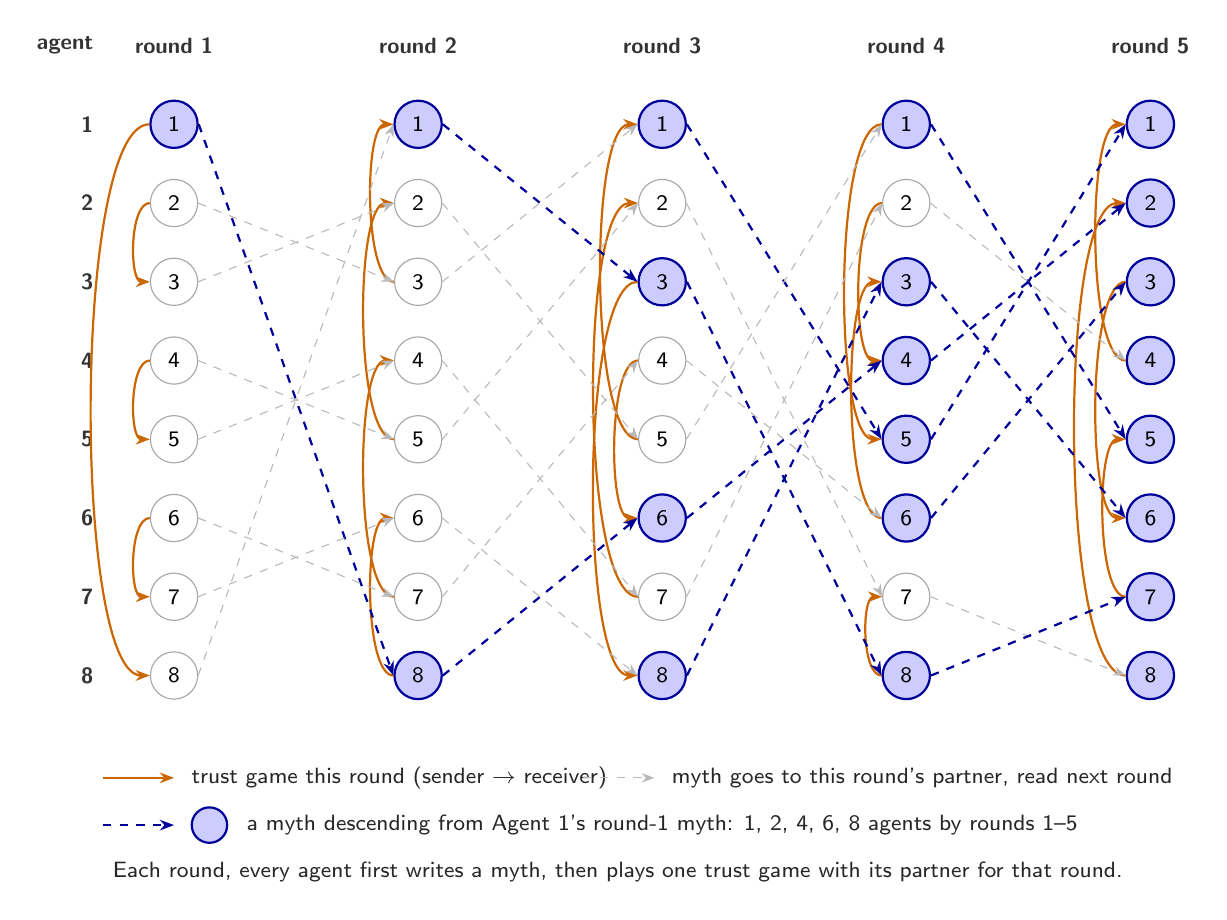
\begin{tikzpicture}[
  font=\small,
  ag/.style={circle, draw=gray!70, fill=white, minimum size=6mm, inner sep=0pt, font=\footnotesize},
  carrier/.style={ag, draw=blue!60!black, fill=blue!20, thick},
  game/.style={orange!80!black, thick, ->, >={Stealth[length=1.8mm]}},
  hop/.style={gray!55, dashed, ->, >={Stealth[length=1.6mm]}},
  carry/.style={blue!60!black, thick, dashed, ->, >={Stealth[length=1.8mm]}},
  lab/.style={font=\footnotesize\bfseries, text=gray!40!black},
  note/.style={font=\footnotesize, text=gray!30!black, align=left},
]
\node[lab] at (0.00,8.0) {round 1};
\node[lab] at (3.10,8.0) {round 2};
\node[lab] at (6.20,8.0) {round 3};
\node[lab] at (9.30,8.0) {round 4};
\node[lab] at (12.40,8.0) {round 5};
\node[lab, anchor=east] at (-0.9,8.0) {agent};
\node[lab, anchor=east] at (-0.9,7) {1};
\node[lab, anchor=east] at (-0.9,6) {2};
\node[lab, anchor=east] at (-0.9,5) {3};
\node[lab, anchor=east] at (-0.9,4) {4};
\node[lab, anchor=east] at (-0.9,3) {5};
\node[lab, anchor=east] at (-0.9,2) {6};
\node[lab, anchor=east] at (-0.9,1) {7};
\node[lab, anchor=east] at (-0.9,0) {8};
\node[carrier] (n11) at (0.00,7) {1};
\node[ag] (n12) at (0.00,6) {2};
\node[ag] (n13) at (0.00,5) {3};
\node[ag] (n14) at (0.00,4) {4};
\node[ag] (n15) at (0.00,3) {5};
\node[ag] (n16) at (0.00,2) {6};
\node[ag] (n17) at (0.00,1) {7};
\node[ag] (n18) at (0.00,0) {8};
\node[carrier] (n21) at (3.10,7) {1};
\node[ag] (n22) at (3.10,6) {2};
\node[ag] (n23) at (3.10,5) {3};
\node[ag] (n24) at (3.10,4) {4};
\node[ag] (n25) at (3.10,3) {5};
\node[ag] (n26) at (3.10,2) {6};
\node[ag] (n27) at (3.10,1) {7};
\node[carrier] (n28) at (3.10,0) {8};
\node[carrier] (n31) at (6.20,7) {1};
\node[ag] (n32) at (6.20,6) {2};
\node[carrier] (n33) at (6.20,5) {3};
\node[ag] (n34) at (6.20,4) {4};
\node[ag] (n35) at (6.20,3) {5};
\node[carrier] (n36) at (6.20,2) {6};
\node[ag] (n37) at (6.20,1) {7};
\node[carrier] (n38) at (6.20,0) {8};
\node[carrier] (n41) at (9.30,7) {1};
\node[ag] (n42) at (9.30,6) {2};
\node[carrier] (n43) at (9.30,5) {3};
\node[carrier] (n44) at (9.30,4) {4};
\node[carrier] (n45) at (9.30,3) {5};
\node[carrier] (n46) at (9.30,2) {6};
\node[ag] (n47) at (9.30,1) {7};
\node[carrier] (n48) at (9.30,0) {8};
\node[carrier] (n51) at (12.40,7) {1};
\node[carrier] (n52) at (12.40,6) {2};
\node[carrier] (n53) at (12.40,5) {3};
\node[carrier] (n54) at (12.40,4) {4};
\node[carrier] (n55) at (12.40,3) {5};
\node[carrier] (n56) at (12.40,2) {6};
\node[carrier] (n57) at (12.40,1) {7};
\node[carrier] (n58) at (12.40,0) {8};
\draw[game] (n14.west) .. controls (-0.57,4.00) and (-0.57,3.00) .. (n15.west);
\draw[game] (n16.west) .. controls (-0.57,2.00) and (-0.57,1.00) .. (n17.west);
\draw[game] (n11.west) .. controls (-1.29,7.00) and (-1.29,0.00) .. (n18.west);
\draw[game] (n12.west) .. controls (-0.57,6.00) and (-0.57,5.00) .. (n13.west);
\draw[game] (n23.west) .. controls (2.41,5.00) and (2.41,7.00) .. (n21.west);
\draw[game] (n27.west) .. controls (2.29,1.00) and (2.29,4.00) .. (n24.west);
\draw[game] (n25.west) .. controls (2.29,3.00) and (2.29,6.00) .. (n22.west);
\draw[game] (n28.west) .. controls (2.41,0.00) and (2.41,2.00) .. (n26.west);
\draw[game] (n33.west) .. controls (5.15,5.00) and (5.15,0.00) .. (n38.west);
\draw[game] (n34.west) .. controls (5.51,4.00) and (5.51,2.00) .. (n36.west);
\draw[game] (n37.west) .. controls (5.15,1.00) and (5.15,6.00) .. (n32.west);
\draw[game] (n35.west) .. controls (5.27,3.00) and (5.27,7.00) .. (n31.west);
\draw[game] (n42.west) .. controls (8.61,6.00) and (8.61,4.00) .. (n44.west);
\draw[game] (n48.west) .. controls (8.73,0.00) and (8.73,1.00) .. (n47.west);
\draw[game] (n46.west) .. controls (8.49,2.00) and (8.49,5.00) .. (n43.west);
\draw[game] (n41.west) .. controls (8.37,7.00) and (8.37,3.00) .. (n45.west);
\draw[game] (n54.west) .. controls (11.59,4.00) and (11.59,7.00) .. (n51.west);
\draw[game] (n58.west) .. controls (11.23,0.00) and (11.23,6.00) .. (n52.west);
\draw[game] (n53.west) .. controls (11.59,5.00) and (11.59,2.00) .. (n56.west);
\draw[game] (n57.west) .. controls (11.71,1.00) and (11.71,3.00) .. (n55.west);
\draw[carry] (n11.east) -- (n28.west);
\draw[hop] (n12.east) -- (n23.west);
\draw[hop] (n13.east) -- (n22.west);
\draw[hop] (n14.east) -- (n25.west);
\draw[hop] (n15.east) -- (n24.west);
\draw[hop] (n16.east) -- (n27.west);
\draw[hop] (n17.east) -- (n26.west);
\draw[hop] (n18.east) -- (n21.west);
\draw[carry] (n21.east) -- (n33.west);
\draw[hop] (n22.east) -- (n35.west);
\draw[hop] (n23.east) -- (n31.west);
\draw[hop] (n24.east) -- (n37.west);
\draw[hop] (n25.east) -- (n32.west);
\draw[hop] (n26.east) -- (n38.west);
\draw[hop] (n27.east) -- (n34.west);
\draw[carry] (n28.east) -- (n36.west);
\draw[carry] (n31.east) -- (n45.west);
\draw[hop] (n32.east) -- (n47.west);
\draw[carry] (n33.east) -- (n48.west);
\draw[hop] (n34.east) -- (n46.west);
\draw[hop] (n35.east) -- (n41.west);
\draw[carry] (n36.east) -- (n44.west);
\draw[hop] (n37.east) -- (n42.west);
\draw[carry] (n38.east) -- (n43.west);
\draw[carry] (n41.east) -- (n55.west);
\draw[hop] (n42.east) -- (n54.west);
\draw[carry] (n43.east) -- (n56.west);
\draw[carry] (n44.east) -- (n52.west);
\draw[carry] (n45.east) -- (n51.west);
\draw[carry] (n46.east) -- (n53.west);
\draw[hop] (n47.east) -- (n58.west);
\draw[carry] (n48.east) -- (n57.west);
\draw[game] (-0.9,-1.3) -- (0.0,-1.3); \node[note, anchor=west] at (0.1,-1.3) {trust game this round (sender $\to$ receiver)};
\draw[hop] (5.2,-1.3) -- (6.1,-1.3); \node[note, anchor=west] at (6.2,-1.3) {myth goes to this round's partner, read next round};
\draw[carry] (-0.9,-1.9) -- (0.0,-1.9); \node[carrier, minimum size=4.5mm] at (0.45,-1.9) {}; \node[note, anchor=west] at (0.8,-1.9) {a myth descending from Agent 1's round-1 myth: 1, 2, 4, 6, 8 agents by rounds 1--5};
\node[note, anchor=west] at (-0.9,-2.5) {Each round, every agent first writes a myth, then plays one trust game with its partner for that round.};
\end{tikzpicture}
\end{document}
